\documentclass[12pt]{article}

\usepackage{graphicx}

\usepackage[margin=1in,dvips]{geometry}

\usepackage{deluxetable}

\newcommand{\commissdate}{Fall 2012}
\newcommand{\surveyproper}{Spring 2013}
\newcommand{\devauc}{De Vaucouleurs'}

% Get rid of the normal page numbers
%\usepackage{nopageno}

% Now use fancyhdr but only to clear the headers and put a page number in the
% upper right

%\usepackage{fancyhdr}
%\pagestyle{fancy}
%\rhead{}
%\rfoot{}
%\lfoot{}
%\cfoot{\thepage}
%\renewcommand{\headrulewidth}{0.0pt}

% for comments
\usepackage{verbatim}


% bibliography stuff
\usepackage{natbib}
% Stripped some defs out of aastex
% plotting
\def\eps@scaling{1.0}% 
\newcommand\epsscale[1]{\gdef\eps@scaling{#1}}% 

\newcommand\plotone[1]{% 
 \centering 
 \leavevmode 
 \includegraphics[width={\eps@scaling\columnwidth}]{#1}% 
}% 
\newcommand\plottwo[2]{% 
 \centering 
 \leavevmode 
 \columnwidth=.45\columnwidth 
 \includegraphics[width={\eps@scaling\columnwidth}]{#1}% 
 \hfil 
 \includegraphics[width={\eps@scaling\columnwidth}]{#2}% 
}% 
\newcommand\plotfiddle[7]{% 
 \centering 
 \leavevmode 
 \vbox\@to#2{\rule{\z@}{#2}}% 
 \includegraphics[% 
  scale=#4, 
  angle=#3, 
  origin=c 
 ]{#1}% 
}% 


%% journal definitions
\newcommand\aj{\rmfamily{AJ}}% 
          % Astronomical Journal 
\newcommand\araa{\rmfamily{ARA\&A}}% 
          % Annual Review of Astron and Astrophys 
\newcommand\apj{\rmfamily{ApJ}}% 
          % Astrophysical Journal 
\newcommand\apjl{\rmfamily{ApJ}}% 
          % Astrophysical Journal, Letters 
\newcommand\apjs{\rmfamily{ApJS}}% 
          % Astrophysical Journal, Supplement 
\newcommand\ao{\rmfamily{Appl.~Opt.}}% 
          % Applied Optics 
\newcommand\apss{\rmfamily{Ap\&SS}}% 
          % Astrophysics and Space Science 
\newcommand\aap{\rmfamily{A\&A}}% 
          % Astronomy and Astrophysics 
\newcommand\aapr{\rmfamily{A\&A~Rev.}}% 
          % Astronomy and Astrophysics Reviews 
\newcommand\aaps{\rmfamily{A\&AS}}% 
          % Astronomy and Astrophysics, Supplement 
\newcommand\azh{\rmfamily{AZh}}% 
          % Astronomicheskii Zhurnal 
\newcommand\baas{\rmfamily{BAAS}}% 
          % Bulletin of the AAS 
\newcommand\jrasc{\rmfamily{JRASC}}% 
          % Journal of the RAS of Canada 
\newcommand\memras{\rmfamily{MmRAS}}% 
          % Memoirs of the RAS 
\newcommand\mnras{\rmfamily{MNRAS}}% 
          % Monthly Notices of the RAS 
\newcommand\pra{\rmfamily{Phys.~Rev.~A}}% 
          % Physical Review A: General Physics 
\newcommand\prb{\rmfamily{Phys.~Rev.~B}}% 
          % Physical Review B: Solid State 
\newcommand\prc{\rmfamily{Phys.~Rev.~C}}% 
          % Physical Review C 
\newcommand\prd{\rmfamily{Phys.~Rev.~D}}% 
          % Physical Review D 
\newcommand\pre{\rmfamily{Phys.~Rev.~E}}% 
          % Physical Review E 
\newcommand\prl{\rmfamily{Phys.~Rev.~Lett.}}% 
          % Physical Review Letters 
\newcommand\pasp{\rmfamily{PASP}}% 
          % Publications of the ASP 
\newcommand\pasj{\rmfamily{PASJ}}% 
          % Publications of the ASJ 
\newcommand\qjras{\rmfamily{QJRAS}}% 
          % Quarterly Journal of the RAS 
\newcommand\skytel{\rmfamily{S\&T}}% 
          % Sky and Telescope 
\newcommand\solphys{\rmfamily{Sol.~Phys.}}% 
          % Solar Physics 
\newcommand\sovast{\rmfamily{Soviet~Ast.}}% 
          % Soviet Astronomy 
\newcommand\ssr{\rmfamily{Space~Sci.~Rev.}}% 
          % Space Science Reviews 
\newcommand\zap{\rmfamily{ZAp}}% 
          % Zeitschrift fuer Astrophysik 
\newcommand\nat{\rmfamily{Nature}}% 
          % Nature 
\newcommand\iaucirc{\rmfamily{IAU~Circ.}}% 
          % IAU Cirulars 
\newcommand\aplett{\rmfamily{Astrophys.~Lett.}}% 
          % Astrophysics Letters 
\newcommand\apspr{\rmfamily{Astrophys.~Space~Phys.~Res.}}% 
          % Astrophysics Space Physics Research 
\newcommand\bain{\rmfamily{Bull.~Astron.~Inst.~Netherlands}}% 
          % Bulletin Astronomical Institute of the Netherlands 
\newcommand\fcp{\rmfamily{Fund.~Cosmic~Phys.}}% 
          % Fundamental Cosmic Physics 
\newcommand\gca{\rmfamily{Geochim.~Cosmochim.~Acta}}% 
          % Geochimica Cosmochimica Acta 
\newcommand\grl{\rmfamily{Geophys.~Res.~Lett.}}% 
          % Geophysics Research Letters 
\newcommand\jcp{\rmfamily{J.~Chem.~Phys.}}% 
          % Journal of Chemical Physics 
\newcommand\jgr{\rmfamily{J.~Geophys.~Res.}}% 
          % Journal of Geophysics Research 
\newcommand\jqsrt{\rmfamily{J.~Quant.~Spec.~Radiat.~Transf.}}% 
          % Journal of Quantitiative Spectroscopy and Radiative Trasfer 
\newcommand\memsai{\rmfamily{Mem.~Soc.~Astron.~Italiana}}% 
          % Mem. Societa Astronomica Italiana 
\newcommand\nphysa{\rmfamily{Nucl.~Phys.~A}}% 
          % Nuclear Physics A 
\newcommand\physrep{\rmfamily{Phys.~Rep.}}% 
          % Physics Reports 
\newcommand\physscr{\rmfamily{Phys.~Scr}}% 
          % Physica Scripta 
\newcommand\planss{\rmfamily{Planet.~Space~Sci.}}% 
          % Planetary Space Science 
\newcommand\procspie{\rmfamily{Proc.~SPIE}}% 
          % Proceedings of the SPIE 


\let\astap=\aap 
\let\apjlett=\apjl 
\let\apjsupp=\apjs 
\let\applopt=\ao 
\newcommand\phn{\phantom{0}}% 
\newcommand\phd{\phantom{.}}% 
\newcommand\phs{\phantom{$-$}}% 
\newcommand\phm[1]{\phantom{#1}}% 
\let\la=\lesssim            % For Springer A&A compliance... 
\let\ga=\gtrsim 
\newcommand\sq{\mbox{\rlap{$\sqcap$}$\sqcup$}}% 
\newcommand\arcdeg{\mbox{$^\circ$}}% 
\newcommand\arcmin{\mbox{$^\prime$}}% 
\newcommand\arcsec{\mbox{$^{\prime\prime}$}}% 
\newcommand\fd{\mbox{$.\!\!^{\mathrm d}$}}% 
\newcommand\fh{\mbox{$.\!\!^{\mathrm h}$}}% 
\newcommand\fm{\mbox{$.\!\!^{\mathrm m}$}}% 
\newcommand\fs{\mbox{$.\!\!^{\mathrm s}$}}% 
\newcommand\fdg{\mbox{$.\!\!^\circ$}}% 
%\newcommand\farcm@mss{\mbox{$.\mkern-4mu^\prime$}}% 
%\let\farcm\farcm@mss 
%\newcommand\farcs@mss{\mbox{$.\!\!^{\prime\prime}$}}% 
%\let\farcs\farcs@mss 
\newcommand\fp{\mbox{$.\!\!^{\scriptscriptstyle\mathrm p}$}}% 
\newcommand\micron{\mbox{$\mu$m}}% 
\def\farcm@apj{% 
 \mbox{.\kern -0.7ex\raisebox{.9ex}{\scriptsize$\prime$}}% 
}% 
\def\farcs@apj{% 
 \mbox{% 
  \kern  0.13ex.% 
  \kern -0.95ex\raisebox{.9ex}{\scriptsize$\prime\prime$}% 
  \kern -0.1ex% 
 }% 
}% 
\newcommand\case[2]{\mbox{$\frac{#1}{#2}$}}% 
\newcommand\slantfrac{\case}% 
\newcommand\onehalf{\slantfrac{1}{2}}% 
\newcommand\onethird{\slantfrac{1}{3}}% 
\newcommand\twothirds{\slantfrac{2}{3}}% 
\newcommand\onequarter{\slantfrac{1}{4}}% 
\newcommand\threequarters{\slantfrac{3}{4}}% 
\newcommand\ubvr{\mbox{$U\!BV\!R$}}%% UBVR system 
\newcommand\ub{\mbox{$U\!-\!B$}}%   % U-B 
\newcommand\bv{\mbox{$B\!-\!V$}}%   % B-V 
\newcommand\vr{\mbox{$V\!-\!R$}}%   % V-R 
\newcommand\ur{\mbox{$U\!-\!R$}}%   % U-R 
\newcommand\ion[2]{#1$\;${\small\rmfamily\@Roman{#2}}\relax}% 
\newcommand\nodata{ ~$\cdots$~ }% 
\newcommand\diameter{\ooalign{\hfil/\hfil\crcr\mathhexbox20D}}% 
\newcommand\degr{\arcdeg}% 
\newcommand\Sun{\sun}% 
\newcommand\Sol{\sun}% 
\newcommand\sun{\odot}% 
\newcommand\Mercury{\astro{\char1}}% Mercury symbol, "1" 
\newcommand\Venus{\astro{\char2}}% Venus symbol, "2" 
\newcommand\Earth{\earth}% 
\newcommand\Terra{\earth}% 
\newcommand\earth{\oplus}% 
\newcommand\Mars{\astro{\char4}}% Mars symbol, "4" 
\newcommand\Jupiter{\astro{\char5}}% Jupiter symbol, "5" 
\newcommand\Saturn{\astro{\char6}}% Saturn symbol, "6" 
\newcommand\Uranus{\astro{\char7}}% Uranus symbol, "7" 
\newcommand\Neptune{\astro{\char8}}% Neptune symbol, "8" 
\newcommand\Pluto{\astro{\char9}}% Pluo symbol, "9" 
\newcommand\Moon{\astro{\char10}}% Moon symbol, "M" 
\newcommand\Luna{\Moon}% 
\newcommand\Aries{\astro{\char11}}% 
\newcommand\VEq{\Aries}% vernal equinox (Aries) 
\newcommand\Taurus{\astro{\char12}}% 
\newcommand\Gemini{\astro{\char13}}% 
\newcommand\Cancer{\astro{\char14}}% 
\newcommand\Leo{\astro{\char15}}% 
\newcommand\Virgo{\astro{\char16}}% 
\newcommand\Libra{\astro{\char17}}% 
\newcommand\AEq{\Libra}% autumnal equinox (Libra) 
\newcommand\Scorpius{\astro{\char18}}% 
\newcommand\Sagittarius{\astro{\char19}}% 
\newcommand\Capricornus{\astro{\char20}}% 
\newcommand\Aquarius{\astro{\char21}}% 
\newcommand\Pisces{\astro{\char22}}% 


\begin{document}



%\begin{comment}

% The fake FWP
fake fwp page1 for toc
%\setcounter{page}{1}
\addcontentsline{toc}{section}{Field Work Proposal}

\newpage
fake fwp page 2

\newpage
fake fwp page 3
\newpage
fake fwp page 4

\newpage
\addcontentsline{toc}{section}{Cover Page}
fake cover page (5)


% The budget
\newpage
%\setcounter{page}{2}
\addcontentsline{toc}{section}{Budget}
fake budget start page 1 (6)

\newpage
fake budget page 2 (7)
\newpage
fake budget page 3 (8)
\newpage
fake budget page 4 (9)
\newpage
fake budget page 5 (10)
\newpage
fake budget page 6 (11)
\newpage
\addcontentsline{toc}{section}{Budget Explanation}
fake budget page 7 (12)

%\end{comment}




% Title and TOC
\newpage 

%\title{Early Career: Measuring Dark Energy with Gravitational Lensing in 
%the Dark Energy Survey}
%\author{Erin Sheldon\\
%{\normalsize Associate Physicist}\\
%\normalsize{Brookhaven National Laboratory}}
%\date{}
%\maketitle


\tableofcontents

%\begin{center}
%  {\large {\bf Abstract}}
%\end{center}

\newpage

\title{Early Career: Measuring Dark Energy with Gravitational Lensing in 
the Dark Energy Survey}
\author{Erin Sheldon\\
{\normalsize Associate Physicist}\\
\normalsize{Brookhaven National Laboratory}}
\date{}
\maketitle



\addcontentsline{toc}{section}{Abstract}
\begin{center}
\section*{Abstract}
\end{center}

%\begin{abstract}

I propose to analyze data from the Dark Energy Survey (DES) to constrain the
properties of Dark Energy.  My primary focus will be on measuring gravitational
lensing effects to probe the expansion history and growth rate of massive
structures in our universe.  I am a DES ``builder'' with data rights and a
leader of the DES lensing effort.

Dark Energy accelerates the expansion of the universe, dramatically increasing
the volume in comparison to a matter-only universe.  Dark Energy also inhibits
the growth of massive structures under gravitational collapse.  Thus the number
density of massive objects such as galaxy clusters as a function of cosmic time
is directly related to the properties of Dark Energy, in particular the
equation of state parameter $w=$pressure/density.  Critical to using the number
density to constrain cosmology is knowing the masses of the clusters. We will
measure these masses using gravitational lensing.  Using cluster counts,
lensing and other complimentary probes, the DES will measure $w$ to $\sim$3\%.
This program is a natural continuation of my earlier measurements of lensing in
the Sloan Digital Sky Survey (SDSS), which are most sensitive such measurements
to date, and naturally leads to future work on projects such as the Large Scale
Synoptic Telescope\cite{lsstweb}.

DES has entered the commissioning phase.  I am in the final stages of
development of a promising new algorithm to measure lensing effects from
astronomical images.  In addition, in collaboration with Mike Jarvis of UPenn,
I am continuing to test and tune the de-facto algorithm and pipeline for DES.
We are strenuously testing these algorithms using simulations and will soon
begin testing on the commissioning data.

After first light, DES will take data for five years, during which I will
process the data as it arrives and perform analysis to extract Dark Energy
parameters.  These analyses will most likely produce results in three stages:
an early set of results from the first year data, a second set of results after
two or three years when multi-epoch data are available, and a final set of
results from the full data set circa 2017.  The DES survey will produce of
order a petabyte of data which will arrive in a steady stream.  For this work I
will require moderate computing infrastructure and the assistance of a research
associate.

%\end{abstract}

\newpage
\addcontentsline{toc}{section}{Narrative}
\section*{Narrative}
\setcounter{section}{1}
\subsection{Introduction}

%The phenomenon of Dark Energy is one of the unsolved mysteries of our time.
The initial discovery of Dark Energy was made by studying the expansion history
of our universe.  According to General Relativity, a universe containing only
ordinary matter decelerates at late times under its own gravitation, but recent
studies of the brightnesses of distant supernovae indicate that our universe
has begun to accelerate \cite{Riess98,Perlmutter99}.  This can happen if there
is an exotic energy component in our universe with an equation of state
parameter $w$=pressure/density that is less than -1/3.

The observational consequences of a Dark Energy component in our universe are
numerous, but for our purposes the following are most relevant: 1) The
expansion history follows a form quite different from that of a matter only
universe, with a change in the sign of the acceleration at late times from
negative to positive \cite{Carroll92}.  2)  Unlike in a matter-only universe,
the growth history of massive structures through gravitation is no longer
determined solely by the properties of the mass density field and the value of
the present day expansion rate \cite{Haiman01}.  For example, without Dark
Energy, the number density of gravitationally collapsed structures of a given
mass at a given time in history is predictable essentially from the Hubble
expansion constant $H_0$ and low order statistics of the mass field such as the
mean of the density and the variance in the density as a function of scale
(ignoring baryons).  But in the presence of Dark Energy, the volume changes
over time in a dramatically different way and the growth of structures is
inhibited.  The cumulative effects of Dark Energy significantly alter the
predicted number of massive structures in a given volume of space.

Gravitational lensing is particularly well suited to studying this problem
(e.g. \cite{Kaiser98,Hu04}).  Lensing is the apparent bending of light as it
passes massive structures.  The amount of bending depends on the lens mass and
the geometry of the lens-source-observer system.  Thus, measurements of a large
sample of lenses at various cosmological epochs will elucidate the expansion
history of the universe, encoded in the geometry, and the growth history,
encoded in the statistical distribution of the measured masses.  

Lensing is more appropriate for measuring masses in an cosmological context
than other techniques.  The traditional technique of using orbital calculations
and Kepler's laws to infer masses does not work because the timescales are too
long to characterize the orbits. Velocities can only be used in a statistical
way, and require assumptions about the dynamical equilibrium of the systems in
question, which is often dubious on the physical scales of interest.
Furthermore, interpretation based on luminous tracers is complicated by the
ubiquitous presence of another mysterious substance: Dark Matter.  Dark Matter
dominates the mass density field, but because it is collisionless it is
distributed very differently from the luminous matter.  Often there are no
luminous tracers in the relevant regions of space with which to infer masses.
With lensing, one only needs enough background sources with which to
statistically measure the lensing signal.

I propose to use data from the Dark Energy Survey (DES, \cite{DESWhitePaper})
to perform gravitational lensing measurements and infer the properties of Dark
Energy.  I am a DES ``builder'', having worked steadily on the project since
it's inception.  Among other things, this designation brings perpetual data
rights for myself, a postdoc and students.  I am a leader in the DES lensing
effort.  My focus will be primarily on optimal measurement of the gravitational
shear induced in the shapes of galaxies by lensing, and using the shear to
infer statistics of the mass density field, namely the mass associated with
galaxy clusters and the power spectrum of the mass density fluctuations in our
universe. Both of these measurements will be highly sensitive to the properties
of Dark Energy.  Using a combination of techniques, we expect to constrain the
equation of state parameter $w$ to a few percent.  As I will describe below,
this is a natural extension of my earlier work in Gravitational Lensing using
data from the Sloan Digital Sky Survey (SDSS) and will lead naturally to work
on the Large Scale Synoptic Telescope \cite{lsstweb}, in which I am a
participant.

\subsection{Previous Lensing Measurements in the SDSS} \label{sec:sdssold}

Using data from the SDSS \cite{York00}, I have made highly accurate and precise
measurements of gravitational shear. I have used these measurements to estimate
the total mass content (normal and dark) associated with galaxies and clusters
of galaxies
\cite{fis00,Sheldon04,SheldonLensing07,JohnstonLensing07,SheldonM2L07}.  These
high quality measurements are facilitated by the excellent data and processing
software of the SDSS, and our development of interpretational techniques that
can extract masses from complex statistical shear measurements
\cite{JohnstonInvert07}.

In these works we measured the shear from millions of background source
galaxies at various projected distances from foreground lenses, from which we
inferred the radial mass density profile.  Because the signal is very weak, we
additionally averaged the signal over many lenses.  This averaging, while in
principle diluting information about the individual lenses, has the positive
effect of averaging out line of sight projections and ``lumpiness'' in the
lenses, which complicates the interpretation.  This in turn facilitates the
extraction of accurate masses.  Figure \ref{fig:massngals} shows results
from \cite{SheldonLensing07,JohnstonLensing07}. Plotted is mean cluster mass as
a function of the number of galaxies in the cluster.  

%\begin{figure}[ht]
\begin{figure}[p]
\centering
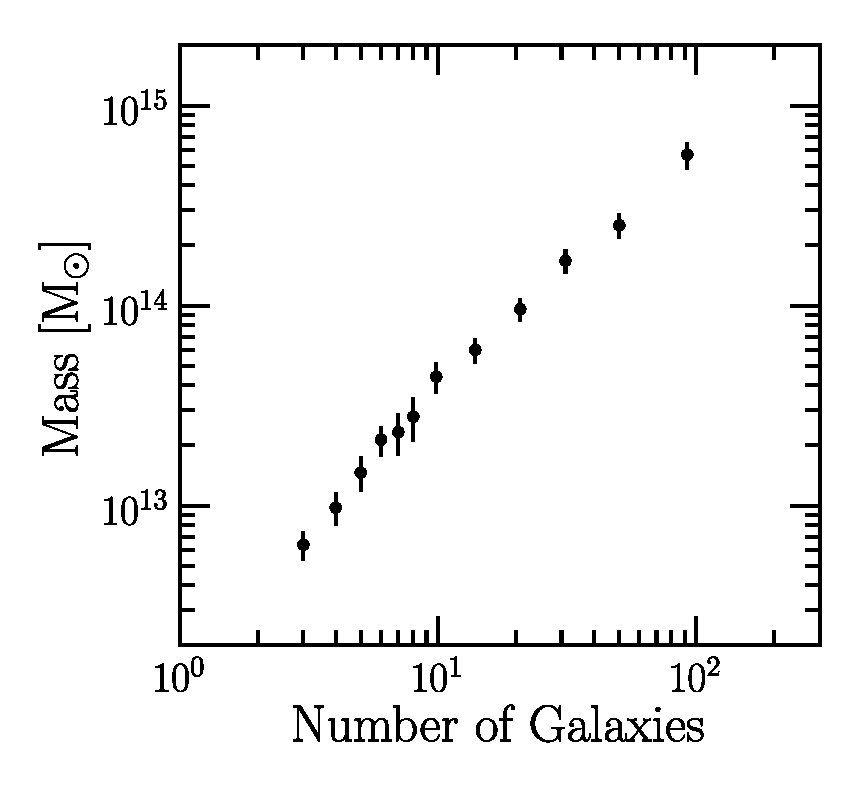
\includegraphics[scale=0.7]{mass-rich-plot.eps}
\caption{Mean cluster mass as a function of the number of
galaxies in the cluster as measured from lensing in SDSS
data \cite{SheldonLensing07,JohnstonLensing07}. This calibration
is critical to measuring Dark Energy with galaxy clusters.\label{fig:massngals}}
\end{figure}



%\begin{figure}[ht] 
\begin{figure}[p] 
\centering 
\includegraphics[scale=0.6]{s8_Om.ps}

\caption{Constraints on the fractional mass density of our universe $\Omega_m$
and the relative variance in the density on 8 Mpc scales $\sigma_8$ as measured
from SDSS data.  These results \cite{RozoCosmo09} are derived by combining the
counts of galaxy clusters with the mass calibrations from gravitational lensing
as shown in Figure \ref{fig:massngals}
\cite{SheldonLensing07,JohnstonLensing07}.  The cluster results break
degeneracies with other probes such as the cosmic microwave background (WMAP).
With DES we will study Dark Energy properties by extending these measurements
back in time.  \label{fig:omegasigma8}} \end{figure}



From galaxy and cluster lensing measurements we confirmed that there is an
enormous amount of unseen dark matter in galaxies, and that this dark matter is
in a ``dark halo'' that extends far beyond the concentrated bundle of stars at
the center of galaxies.  These measurements are completely consistent with the
cold dark matter model.  A number of derived results have come from these basic
measurement papers, in which we have learned a great deal about the connection
between the dark and visible matter in galaxies and clusters, e.g.
\cite{RykoffLXM08,RozoScatter09,TinkerM2N2012}. 

We have also used these measurements to estimate cosmological parameters.  As
stated in the introduction, the number density of halos of a given mass is
related to the mean mass density of the universe and variance in the density.
In \cite{RozoCosmo09} we combined the counts of galaxy clusters with our
lensing mass estimates to constrain these cosmological parameters.  Figure
\ref{fig:omegasigma8} shows results from \cite{RozoCosmo09} constraining the
fractional mass density $\Omega_m$ and the relative variance in mass density on
8 Mpc scales $\sigma_8$.  In \cite{TinkerM2N2012} we use the ratio of mass to
number density in clusters, combined with the large scale clustering of all
galaxies, to place further complimentary constraints on $\Omega_m$ and
$\sigma_8$.  All these results are consistent with one another and the Cold
Dark Matter theory.

While powerful in themselves, these results are also very complimentary to
other measurements, breaking degeneracies in analyses of the Cosmic Microwave
Background \cite{KomatsuWMAPCosmo09}. 

As I will describe in the section on DES, gravitational shear measurements
are central to two of that survey's primary goals.  The techniques we developed
in the SDSS are directly applicable to DES science, especially the study of
galaxy clusters as cosmological probes.  By extending the measurements backward
in time with the deeper DES data, we will learn about Dark Energy as well as
Dark Matter.


\begin{comment}
The lensing statistic I use is the gravitational shear.  Because the path of
light in the absence of lensing is not known, the bending angle is not usually
measurable.  But the difference in the bending angle vector across the face of
a source is measurable because it results in a change in the shape of the
background sources.  The unlensed shape is also not known, but because lensing
causes correlations in the shapes of all the galaxies behind a lens that would
not exist without the lensing effect, one can statistically infer the net
change in shape.  This statistical measurement requires averaging the shapes of
a large number of background galaxies.
\end{comment}

\subsection{New Lensing Shear Measurement Technique}

The weak gravitational shear effect is a very small distortion of the images of
galaxies by foreground mass distributions due to the bending of light.  This
small distortion produces correlations in the ellipticities of the background
galaxies, which can only be measured statistically.  In principle all one needs
is many galaxies to extract this signal.  However, the telescope optics and
atmosphere distort and blur the images of galaxies, and this also produces
correlations in the ellipticities of galaxies; the combined effect is generally
referred to as the point spread function (PSF). The primary affect is a
convolution, which means the effect is more significant for smaller galaxies.
Most detected galaxies are of order the size of the PSF, and the effect is
typically at a level much larger than the lensing effect we wish to measure.

Many methods have been developed to measure and remove the effect of the PSF to
produce unbiased ellipticity measurements, e.g.
\cite{ksb95,Bern02,Miller07,Melchior11} and many more.  No method yet tested
has proven good enough to meet the DES survey requirements for realistic galaxy
populations:  calibration errors of 0.004 in the measured shear, and additive
errors 0.0004.

I have been developing a new technique that shows promise to deliver on the DES
requirements.  The method uses mixtures of gaussians to represent the galaxies
and PSF, and bayesian techniques to control noise bias.  This model has enough
flexibility to represent the canonical galaxy types; this has been
independently verified recently \citep{HoggGMix12}.  One result of my recent
research is that many fewer gaussians are required than used in
\cite{HoggGMix12} when the object is of order the size of the PSF; three is
enough.  When also demanding the Gaussians are co-centric and co-elliptical the
parameter space is reduced even further.  

It is tempting to just use the canonical galaxy profiles (exponential disks and
$exp(-r^{1/4})$ ``\devauc'' profiles) to fit for the ellipticity, but these are
computationally intensive to generate when convolving with a PSF and the pixel
response.  Using Gaussians greatly speeds up the convolution and model
generating process; this is important for controlling the noise bias described
below.

Other features of the method are more generic and are designed to mitigate the
effects of noise.  Noise is known to produces bias in the ellipticity
measurement when using either maximum likelihood \cite{Refreg12} or the full
expectation value \cite{Miller12}.  This can be mitigated using the techniques
in \cite{Miller07,Miller12}, which involve using prior information on the
ellipticity and size distributions of the galaxy population as a whole.  Use of
the prior on ellipticity was introduced in \cite{Miller07} and I developed the
use of the size prior distribution independently of \cite{Miller12}.  I have
developed an alternative method to implement these ideas using a Monte Carlo
Markov Chain, and the code is publicly available (the code used for \cite{Miller07}
is proprietary).

The results using simulations are quite promising.  For exponential disk galaxies,
a prior on the ellipticity distribution is sufficient, as shown in figure \ref{fig:get}


\begin{figure}[p]
\centering

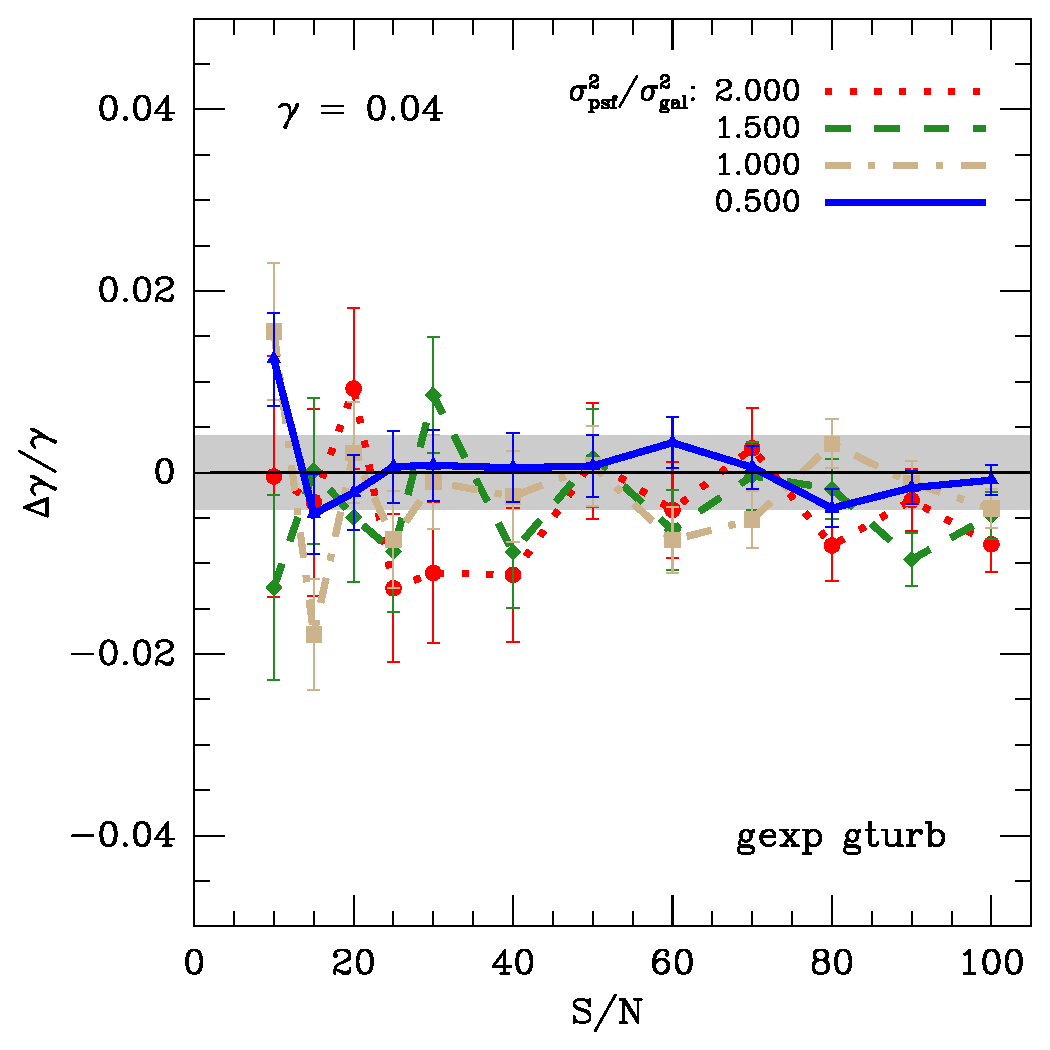
\includegraphics[scale=0.4]{mcbayes-get01r05r06r07r08-yr-0.050-0.050-frac.eps}
\caption{Shear bias as a function of signal-to-noise ratio (S/N) for exponential disk
galaxies fit by a Gaussian mixture.  The different line/point styles represent
galaxies of different size ratio with respect to the point spread function.
A prior on the distribution of ellipticities has been applied.
The gray band is the DES requirement on the shear error; the error is within
the DES requirements for S/N $\geq$ 20 and for galaxies comparable to
or larger than the PSF\label{fig:get}}


\end{figure}



\begin{figure}[p]
\centering

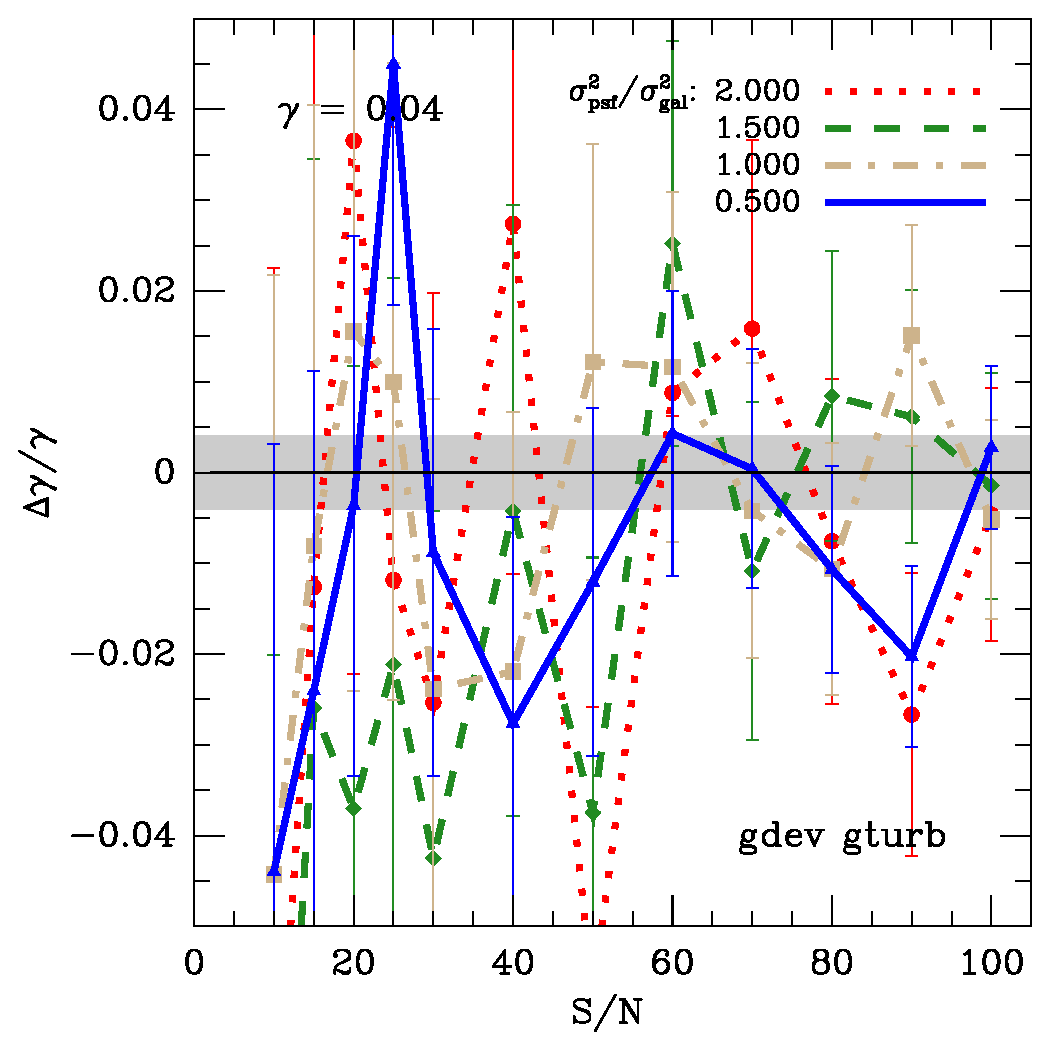
\includegraphics[scale=0.4]{mcbayes-gdt02r11-yr-0.050-0.050-frac.eps}
\caption{Shear bias as a function of signal-to-noise ratio (S/N) for
$exp(-r^{1/4})$ galaxies fit by a Gaussian mixture.  The lines and shaded area
are the same as figure \ref{fig:get}. Measurements of these galaxy types are
intrinsically more noisy than exponential disks, and at the current writing
more statistics are needed to fully characterize the error.  In addition to a
prior on ellipticity, a prior on the distribution of sizes is applied. The
error is within the DES requirements.  A topic of future research will be to
determine the priors from data \label{fig:gdt}}


\end{figure}

\subsection{The Dark Energy Survey (DES)}

The Dark Energy Survey (DES) is an optical, multi-band survey of 5000 square
degrees using the 4-meter ``Blanco'' telescope at the Cerro Tololo
Inter-American Observatory in Chile. A new camera is being built and the
telescope repaired and upgraded.  The DES will utilize gravitational lensing,
an optical cluster survey, supernovae, and galaxy clustering to constrain the
properties of Dark Energy.  Combining DES lensing measurements and DES optical
observations of galaxy clusters with observations by the South Pole Telescope
(SPT, \cite{SPT04}) of the same galaxy clusters, greatly enhances the
constraining power.  These combined methods will constrain the Dark Energy
equation of state parameter $w$ to better than 3\%.  First light is planned for
\commissdate, and the survey will run for five years.  DES operations are
funded in part by the U.S.  Department of Energy. 


The SPT will use the Sunyaev-Zel'dovich (SZ) Effect \cite{Birkinshaw99}, the
Compton up-scattering of light from the cosmic microwave background by the hot
gas in galaxy clusters, to find a complete sample of clusters to high redshift.
This cluster sample has selection that is complimentary to the DES optical
cluster selection in that it is expected to be nearly independent of the
distance of the cluster from the observer.  As with DES, the goal of the SPT is
to use these clusters to probe the growth of structure, and the volume of
space, as a function of time in order to constrain Dark Energy.  Since it is
the number density of clusters of a given mass that is sensitive to Dark
Energy, an important part of each cluster survey will be the calibration of the
mass-observable relationship via lensing.  In \S \ref{sec:deslensing} I will
describe in detail our plans for measuring this relationship using DES optical
data.

In addition to galaxy clusters, the DES will use a number of other probes to
constrain Dark Energy properties.  These include two other lensing probes:
Shear-shear correlations as a function of scale and the cross-correlation
between shear and known objects as a function of scale.  Data are shared
between cluster mass measurements and these probes, but because the correlation
functions cover a much larger range of scales, they are complimentary.  There
is also a Supernova program that, while less constraining by itself, breaks
degeneracies between certain cosmological parameters.  

Table \ref{table:constraints} shows forcasted constraints on $w$ for various
techniques employed by DES \cite{DESWhitePaper}.  These forecasts are for DES
and SPT data alone; combining with other data, for example from cosmic
microwave background measurements from the Planck satellite
\cite{PlanckBluebook}, can significantly increase the precision of certain
probes.

\begin{deluxetable}{ll}
\tablecaption{Projected DES Constraints on Constant $w$ Dark Energy Models.
\label{table:constraints}}
\tablewidth{0pt}
\tablehead{
	\multicolumn{1}{l}{Method} &
	\colhead{$\sigma_w$}
}
\startdata
Clusters &  \\
~~~Abundance & 0.13  \\
~~~with WL Calibration & 0.09 \\
Weak Lensing & \\
~~~Cosmic Shear (CS) & 0.15  \\
~~~Galaxy/Cluster-shear(GS) + Angular Clustering(AC) & 0.08  \\
~~~CS + GS + AC & 0.03  \\
Angular Clustering of Galaxies & 0.36 \\
Supernovae Ia & 0.34 \\
\enddata
\end{deluxetable}




\subsection{Lensing Analysis of DES Data} \label{sec:deslensing}

\subsubsection{Science Analysis}

In collaboration with Mike Jarvis and Bhuvnesh Jain of Penn, I am working to
create data processing pipelines and analysis codes to measure gravitational
lensing in DES.  I will use this data to calibrate the masses of the galaxy
clusters used in the cosmological analyses.  I will also participate in the
measurement of shear-shear correlations (cosmic shear).  These are critical
components of the DES mission.

As described in the introduction, the cosmological information from clusters is
primarily in the number density of clusters with a given mass as a function of
time.  Clusters are identified not by their mass but by other indicators, such
as the SZ effect from SPT data or by the clustering of visible galaxies in DES
imaging data.  The strength of the SZ effect and the number of galaxies are
both correlated with mass, but that correlation must be measured by a secondary
method.  As described in the introduction, lensing is the best method for doing
this.  

As described in \S\ref{sec:sdssold}, in our studies of SDSS lensing we have
developed analysis techniques to calibrate the mass-observable relation of
clusters (Figure \ref{fig:massngals}).  Using this calibration in conjunction
with the number density we have inferred cosmological parameters (Figure
\ref{fig:omegasigma8}).  These techniques are limited only by our understanding
of the systematics and characterization of the cluster selection process.  The
volume and depth of DES is sufficiently large to perform equivalent
measurements in many bins of cosmic time.  Time dependent measurements will
allow us to extend our cosmological analysis to constrain the properties of
Dark Energy.

In contrast with cluster lensing measurements, cosmic shear is the correlation
of shears across the sky independent of the location of foreground structures.
Since the shear is related to mass, the cosmic shear can be used to directly
infer statistics of the underlying mass distribution, the evolution of which is
directly related to the properties of Dark Energy.  Because the signal need not
be modeled in terms of cluster halos, the interpretation of cosmic shear can be
simpler than cluster lensing.  However, the measurement involves directly
correlating shears from many sources as a function of their separation on the
sky, which can propagate systematic errors directly into the measurement. Thus
cosmic shear and cluster lensing are quite complimentary.



Table \ref{table:constraints} shows the power of lensing in the DES to
constrain $w$ as compared to other DES probes.

%\lhead{}
\subsubsection{Data Reduction and Removal of Systematic Effects} 
\label{sec:des:process}

Gravitational Shear alters the shapes of galaxy images, producing recognizable
patterns in their ellipticities across the sky. Thus accurate shear
measurements require accurate measurements of galaxy shapes.  But there are a
number of factors other than lensing that must be taken into account in order
to extract shear signal from the shapes of galaxies. In fact these other
factors are typically 10 to 100 times larger than the shear signal.

The most dominant source of error is the intrinsic shape of the galaxy itself.
While the shear may alter the ellipticity of a galaxy by less than a percent
(the smallest shears measured in \cite{SheldonLensing07} are $10^{-4}$!) the
typical galaxy ellipticity is about 0.3.  It is impossible to measure typical
shears from a single galaxy image.  However, this ``shape noise'' is purely
random, so with enough galaxies the shear signal can be extracted using
statistical techniques.

Other effects are less benign and must be explicitly corrected.  The most
serious of these is the point spread function (PSF) of the sky plus telescope
optical system. The sky causes enough blurring of images to significantly alter
the shapes of most galaxies, diluting the shear signal.  Furthermore the
optical system and instrument will significantly distort and blur the shapes of
objects, producing correlations in their shapes that can mimic lensing.

There are existing techniques for removing these effects but for DES Mike
Jarvis and I are developing a new pipeline designed to be nearly optimal in
tracking the PSF and accounting for its effects in the shear estimation
\cite{Bern02,JarvisJain04}.  Furthermore, this pipeline can make full use of
the multi-epoch DES data where the sky is observed many times.  A prototype of
this ``multishear'' pipeline is already in place and is being tested on
simulated DES data.  This pipeline will continue to undergo heavy testing and
refinement in preparation for commissioning in Spring 2012.  We will further
test this pipeline in a real world setting using the multi-epoch southern SDSS
survey as described in section \S \ref{sec:sdssnew}.  After the survey comes
online in \commissdate, we will process the data in real time as it arrives.
The processing of simulated and real data will require significant manpower and
computing resources.

\subsection{New Analysis of SDSS Multi-epoch Data} \label{sec:sdssnew}

Once the pipeline described in \S \ref{sec:des:process} reaches a state of
maturity, we will process the multi-epoch data from the SDSS ``southern
stripe''.  Although this data is only 225 square degrees and somewhat shallower
than the final DES data, it is interesting both for testing our pipeline and
performing a cosmological analysis.  The data will be a more stringent test of
the pipeline than DES in the sense that there are many more epochs, typically
30-40.  This means many of the galaxies we use will have no detection at all on
the single epoch images, requiring the multishear code to deal properly with
very noisy data.  But it is an excellent data set for a lensing analysis as
well, being comparable or larger in volume than any existing cosmic shear
study.  I expect at least one publication on cosmological parameters will be
based on this work.

\subsection{BOSS and LSST}

I am an ``architect'' of the Baryon Oscillation Spectroscopic Survey (BOSS,
\cite{BossWhitePaper}), leading the spectroscopic target selection.  I am also
a member of LSST, working on the early stages of lensing pipeline development.
Although no equipment purchases or additional manpower are required to support
this work, I am contributing a total of 25\% of my time to these two projects.

\subsection{Requested Resources}

\subsubsection{Computing}

We will commission the DES survey in \commissdate\ and run for five years,
generating about a petabyte of data in total.  For lensing we will process all
the reduced single-epoch images and multi-epoch images, which amount to about
130 terabytes.  We must assemble more storage in preparation for the survey
data.

In order to process the data as it arrives we will also require significant
manpower and computing resources.  The NSF funded DES data management (DESDM)
is committed to produce a single processing of the data per year.  Thus,
although our lensing pipelines will be incorporated into DESDM, all development
and testing must occur outside of DESDM.  

In order to test our pipelines and analysis codes we must process the full data
set many times.  This is because many systematics tests require essentially
the full data set to explore.  And only from analyzing the full data set to
extract the lensing signal will we be able to feed back what we have learned
into the pipelines.  Working with a single processing would be highly
restrictive.  Thus we must have our own separate computing resources to
facilitate these tests and analyses.  

We projected our current running times, and expect it would take about 2.5
weeks to process the final DES data on a moderate 70 node cluster with at least
8 cores per node and 4 GB of memory per core.  These  numbers assume 2015
computer speeds, which will be the ``average'' speed for our computers
purchased over the five year period. This is approximately the desired
processing time given that we want to reprocess the data with several
iterations on two or more independent shape algorithms in order to obtain a
robust result.

We will also require significant resources for the science analysis, which is
computationally intensive.  As a reference point, the SDSS analysis presented
in \S \ref{sec:sdssold} required running for a week on a cluster of 80
processors.  The mass and luminosity analysis of \cite{SheldonM2L07} is even
more intensive, requiring two weeks on a 300 processor cluster (although these
processors were a factor of two slower than the current generation).  The DES
data set will be 50 times larger.

Because of Moore's law, and the steady data flow we expect, it makes sense to
buy the computing over a period of time with most purchases toward the end of
the survey.  To store and process the DES images, we propose to spend about
\$31,000/year for five years (2012-2016), accruing about 130TB of storage per
year plus processing nodes.  The first year we will acquire around 14TB of
storage and about 15 nodes with at least 4GB of memory per core and at least 8
cores.  Or reference spec is 26kSI2k, 104 HEP-SPEC 2006 .  In following years
we will purchase more disk and CPU for the same price, and keep a trajectory to
our goal.  We expect to assemble a system with about 70 actual nodes, which is
about 120 units of our spec.  An outline of our plans for computing purchases
is shown in Table \ref{table:computing}.

Note these prices include bulk discounts from purchasing along with other
experiments through the RHIC-Atlas Computing Facility at BNL.  

\begin{deluxetable}{lcc}
    \tabletypesize{\small}
    \tablecaption{Projected Computing Purchases\label{table:computing}}
    \tablewidth{0pt}
    \tablehead{
        \multicolumn{1}{l}{Fiscal Year} &
        \colhead{Compute Servers with 2 GPUs}   & 
        \colhead{Total Storage} \\
        &
        &
        [TB]
    }
    \startdata
2013 & 2 & 26 \\
2014 & 2 & 26 \\
2015 & 2 & 26 \\
2016 & 2 & 26 \\
2017 & 2 & 26 \\
\hline
\relax\\[-1.7ex]
Total in 5 years & 10 & 130 TB \\\\[-2.7ex]
\enddata

    \tablecomments{The number of compute nodes purchased is based on the
    assumption that each node and GPU (Intel 12 cores, 32GB ram, two nvidia
    2050 GPUS) would stay at the performance level of a node purchased in 2012.
    It is not clear how the performance per GPU will increase over time so this
    table is conservative.  Disk is likely to get cheaper, so the 13TB per
    machine could be expanded at fixed cost. Power, cooling and maintenance
    will be provided at no extra cost to this experiment, but overhead 
    and slight escalation are included in the budget.}

    \end{deluxetable}
    


\subsubsection{Research Associate}

We plan for much of the higher level analysis and many of the science papers to
be led by research associates (postdocs).  We expect to hire a postdoc during
the first year of the award for three years and a second postdoc to begin in
the fourth year.  The work of these postdocs would focus on the measurement of
shear statistics, testing, and interpretation in terms of mass and cosmology.  

\subsubsection{Salary and Travel}

We ask for 100\%  of Erin Sheldon's salary and overhead for five years, and
100\% for a research associate for five years.

The remaining funds are primarily for travel expenses.   The DES collaboration
is multi-national and Erin Sheldon and a postdoc will most likely travel abroad
to the collaboration meetings.  Sheldon plans to spend three weeks each summer
at a workshop in the US, such as those held at Aspen and Santa Fe.  Further
travel will involve attending a few conferences per year across the US for both
Sheldon and postdoc.  Erin Sheldon will also make regular trips to the
University of Pennsylvania to collaborate with Mike Jarvis and Bhuvnesh Jain.

\clearpage
\newpage
\subsection{Timeline}

This is an outline of the activities for the five year extent of the award.  It
is assumed that the primary collaborators on these activities are Erin Sheldon
(ES) of BNL, Zhaoming Ma (ZM) of BNL, and research associates to be hired in
the Fall of 2012 and 2015.  Zhaoming may continue working on the project after
he leaves BNL in fall 2012.

\begin{itemize}

\item {\bf Fall 2011-Early Spring 2012} Continued testing of the weak lensing
pipeline on simulated DES data (ES, ZM).  Processing of full DES
simulated data set for DES data challenge 6 (ES).     Continued development of
PSF interpolation code (ZM).

\item {\bf Spring \& Early Summer 2012} Process and evaluate commissioning data
as it arrives.  (ES,ZM)

\item {\bf Late Summer \& Fall 2012} Survey proper begins; process data as it
arrives.  Re-process data as bugs are found and algorithms improve. (ES,ZM).
Begin science lensing analysis (ES).  ZM departs, new postdoc arrives, staying
through Fall 2015.

\item {\bf Fall 2013} Publication of first year DES measurements for
galaxy and cluster-mass correlations (ES).  

\item {\bf 2014} Continue processing data as it arrives (ES).  Continue
improving algorithms (ES).  Postdoc hire working on own science projects and
image processing.  First publications using multi-epoch data (ES,postdoc) in
2014.

\item {\bf 2015-2017}  Activities should continue as before until survey end.
Processing data as it arrives, incrementally improving the data pipelines and
analysis codes.  Analysis methods will evolve, especially as the final data are
in hand and there are many epochs with which to work.   There will be
intermediate publications based on this data.  New postdoc hire will arrive
in Fall 2015.

\item {\bf Post survey} A re-processing of all data through the final pipelines
and final analysis of the full dataset to extract cosmological information (ES,postdoc).


\end{itemize}







\newpage
\addcontentsline{toc}{section}{Appendix 1: Biographical Sketch}
\section*{Appendix 1: Biographical Sketch}

%\setlength{\oddsidemargin}{-0.1in}
%\setlength{\evensidemargin}{-0.1in}
%\setlength{\textwidth}{6.7in}
%\setlength{\topmargin}{-0.25in}
%\setlength{\textheight}{9.0in}

\newcommand{\tsp}{\vspace{0.1cm}}
\newcommand{\isp}{\vspace{0.3cm}}
\newcommand{\ssp}{\vspace{0.4cm}}


{\Large {\bf Erin Sheldon}}
\tsp
%
% Address information.
%

\noindent
Bldg 510

\noindent
Brookhaven National Laboratory

\noindent
Upton, NY 11973

\noindent
(631) 344-3117

\noindent
erin.sheldon@gmail.com

\newcommand{\myshorttab}{0.5in}
\newcommand{\mytab}{0.75in}
\newcommand{\mylongtab}{1.25in}

\vspace{0.4cm}
\noindent
\makebox[1.25in][l]{{\large \bf Education and Training}}{}
\vspace{0.2cm}
\newline
\makebox[\mytab][l]{}{Postdoctoral Fellow, Center for Cosmology and Particle Physics}
\newline
\makebox[\mylongtab][l]{}{~~~~~~~~~~~~~~~~~~~~~~~~~~~~~{\bf New York University}}
    \hfill
    \makebox[1in][r]{{\small \it Sep 2005--Sep 2008}}
\newline
\makebox[\mytab][l]{}{Postdoctoral Fellow, Kavli Institute for Cosmological Physics}
	\newline
\makebox[\mylongtab][l]{}{~~~~~~~~~~~~~~~~~~~~~~~~~~~~~{\bf University of Chicago}}
	\hfill
	\makebox[1in][r]{{\small \it Aug 2002--Aug 2005}}
\newline
\makebox[\mytab][l]{}{Research Assistant, {\bf FNAL}}
	\hfill
	\makebox[1in][r]{\small \it Jun 1998--Sep 1998}
\newline
\tsp
\noindent
\makebox[\mytab][l]{}{Ph.D., {\bf University of Michigan}}
    \hfill
    \makebox[1in][r]{\small \it Sep 1997--Aug 2002}
\newline
\tsp
\makebox[\mytab][l]{}{B.S., {\bf University of Missouri}}
\hfill
\makebox[1in][r]{\small \it Aug 1992 -- May 1997}


%
% Experience...
%

\vspace{0.4cm}
\noindent
\makebox[1.25in][l]{{\large \bf Experience}}{}
\newline
\vspace{0.2cm}
\makebox[\mytab][l]{}{Associate Physicist, {\bf Brookhaven National Laboratory}}
\newline
\makebox[1.25in][l]{}{}
        \hfill
        \makebox[1in][r]{{\small \it September 2008--present}}

\vspace{0.3cm}
\noindent
\makebox[1.25in][l]{{\large \bf Graduate and Postdoctoral Advisors and Advisees}}{}
\vspace{0.2cm}
\newline
\makebox[\myshorttab][l]{}{{\large \bf Advisors}}
\newline
\makebox[\mytab][l]{}{Postdoctoral Advisor: David Hogg, New York University}
\newline
\makebox[\mytab][l]{}{Postdoctoral Advisor: Josh Frieman, University of Chicago}
\newline
\makebox[\mytab][l]{}{Thesis Advisor: Timothy McKay, University of Michigan}
\newline
\makebox[\myshorttab][l]{}{{\large \bf Advisees}}
\newline
\makebox[\mytab][l]{}{Postdoc, BNL: Zhaoming Ma}


%\noindent
%\makebox[1.25in][l]{}
%\parbox{5.40in}{
%Ph.D., Physics\newline
%Thesis advisor: Prof. Timothy McKay\newline
%Title of thesis: ``Galaxies, Luminosity, and Mass: Gravitational Lensing Measurements of the Correlation between Dark and Luminous Matter''
%}




\newpage
\vspace{0.2in}
\noindent
\newline
\newline
{\Large {\bf Selected Publications for Erin Sheldon} }
\newline
Note Appendix 3 holds the references for the narrative. 
\vspace{4mm}

\begin{tabular}{p{3mm} p{5.5in}}

1 & E.~S. {Sheldon} et~al.
\newblock {Photometric Redshift Probability Distributions for Galaxies in the SDSS DR8}.
\newblock {\em arXiv:1109.5192},  September 2011. \\[6pt]

2 & J. {Tinker}, E.~S. {Sheldon} et~al.
\newblock {Cosmological Constraints from Galaxy Clustering and the Mass-to-Number Ratio of Galaxy Clusters}.
\newblock {\em arXiv:1104.1635},  April 2011. \\[6pt]

3 & E. {Rozo} et~al.
\newblock {Cosmological Constraints from the Sloan Digital Sky Survey maxBCG Cluster Catalog}.
\newblock {\em \apj}, 708:645-660, January 2010. \\[6pt]

4 & E.~S. {Sheldon} et~al.
\newblock {Cross-correlation Weak Lensing of SDSS Galaxy Clusters III:
  Mass-to-light Ratios}.
\newblock {\em \apj}, 703:2232-2248, October 2009. \\[6pt]

5 & D.~E. {Johnston}, E.~S. {Sheldon}, et~al.
\newblock {Cross-correlation Weak Lensing of SDSS Galaxy Clusters II: Cluster
  Density Profiles and the Mass--Richness Relation}.
\newblock {\em arXiv:0709.1159}, September 2007. \\[6pt]

6 & E.~S. {Sheldon} et~al.
\newblock {Cross-correlation Weak Lensing of SDSS Galaxy Clusters I:
  Measurements}.
\newblock {\em \apj}, 703:2217-2231, October 2009. \\[6pt]

%5 & B.~P. {Koester} et~al.
%\newblock {A MaxBCG Catalog of 13,823 Galaxy Clusters from the Sloan Digital
%  Sky Survey}.
%\newblock {\em \apj}, 660:239--255, May 2007.\\[6pt]

7 & E.~S. {Sheldon} et~al.
\newblock {The Galaxy-Mass Correlation Function Measured from Weak Lensing in
  the Sloan Digital Sky Survey}.
\newblock {\em \aj}, 127:2544--2564, May 2004.\\[6pt]

%7 & T.~A. {McKay}, E.~S. {Sheldon}, D.~{Johnston}, E.~K. {Grebel}, F.~{Prada},
%  H.-W. {Rix}, N.~A. {Bahcall}, J.~{Brinkmann}, I.~{Csabai}, M.~{Fukugita},
%  D.~Q. {Lamb}, and D.~G. {York}.
%\newblock {Dynamical Confirmation of Sloan Digital Sky Survey Weak-lensing
%  Scaling Laws}.
%\newblock {\em \apjl}, 571:L85--L88, June 2002.\\[6pt]

8 & T.~A. {McKay}, E.~S. {Sheldon}, et~al.
\newblock {Galaxy Mass and Luminosity Scaling Laws Determined by Weak
  Gravitational Lensing}.
\newblock {\em ArXiv Astrophysics e-prints}, August 2001.\\[6pt]

9 & E.~S. {Sheldon} et~al.
\newblock {Weak-Lensing Measurements of 42 SDSS/RASS Galaxy Clusters}.
\newblock {\em \apj}, 554:881--887, June 2001.\\[6pt]

10 & P.~{Fischer}, T.~A. Mckay, E.~S. Sheldon, et~al.
\newblock {Weak Lensing with Sloan Digital Sky Survey Commissioning Data: The
  Galaxy-Mass Correlation Function to 1 Mpc}.
\newblock {\em \aj}, 120:1198--1208, September 2000.

\end{tabular}

\ssp
\ssp
\noindent
\parbox[l]{1.25in}{{\bf Synergistic \\ Activities}}
\parbox[t]{5.40in}{
Elected {\bf Builder} of the Dark Energy Survey \hfill {\small 2011} \newline
Elected {\bf Architect} of the Sloan Digital Sky Survey III \hfill {\small 2011} \newline
}

\newpage

\vspace{0.2in}
\noindent
\newline
\newline
{\Large {\bf Selected Collaborators} }
\newline

\noindent
Blanton, Michael, New York University \newline
Cunha, Carlos, University of Michigan \newline
Dawson, Kyle, University of Utah \newline
Hogg, David, New York University \newline
Ho, Shirley, University of Pittsburgh \newline
Mandelbaum, Rachel,  Carnegie Mellon University \newline
McDonald, Pat, Brookhaven National Laboratory \newline
Myers, Adam, University of Wyoming \newline
Rozo, Eduardo, Kavli Institute for Cosmological Physics \newline
Schlegel, David, Lawrence Berkeley National Laboratory \newline
Slosar, Anze, Brookhaven National Laboratory \newline
Tinker, Jeremy, New York University \newline
Wechsler, Risa, Stanford University \newline
Weinberg, David, Ohio State University \newline
White, Martin, University of California-Berkeley \newline
Zehavi, Idit, Case Western Reserve University \newline



\newpage
\addcontentsline{toc}{section}{Appendix 2: Current and Pending Support}
\section*{Appendix 2: Current and Pending Support}

Dr. Erin S. Sheldon is fully supported by Brookhaven National Laboratory as an
Assistant Physicist in the Astrophysics and Cosmology Group of the Physics
Department at 100\%.  Pending project approval, this support will be reduced
appropriately and redirected to the work proposed herein.  There is no other
support pending.

\begin{table}[h]
\begin{center}
\begin{tabular*}{0.85\textwidth}{ll}
B\&R \#YN010000  & \parbox[t]{\textwidth}{BNL Laboratory Directed 
   Research \& Development \\ Award} \\
                 & LDRD 10-45 (FY 2010 -– FY 2012) \\
                 & Astrophysics \& Cosmology Initiative \\
                 & 100\%
\end{tabular*}
\parbox{0.85\textwidth}{\caption{{\bf Current Funding}: Program Development 
\& Lab Directed Research \& Development \label{table:support}}}
\end{center}
\end{table}



\newpage
\addcontentsline{toc}{section}{Appendix 3: Bibliography for Narrative}
\renewcommand{\refname}{\section*{Appendix 3: Bibliography for Narrative}\label{app:bib}}
\bibliographystyle{unsrt}
\bibliography{astroref}
\vspace{5mm}
\noindent
{\bf Key:} {\it AJ} is The Astronomical Journal, {\it ApJ} is The 
Astrophysical Journal and {\it MNRAS} is The Monthly Notices of the Royal
Astronomical Society.






\newpage
\addcontentsline{toc}{section}{Appendix 4: Facilities and Other Resources}
\section*{Appendix 4: Facilities and Other Resources}

We plan to acquire a large amount of computing.  The housing, power and
cooling, administration, and maintenance for these computers will be provided
by the RHIC-Atlas Computing Facility at Brookhaven National Lab at no additional cost
to this experiment.		

\newpage
\addcontentsline{toc}{section}{Appendix 5: Equipment}
\section*{Appendix 5: Equipment}

The equipment currently available to this project is shared time on a set of 25
compute nodes and a file server purchased in 2009-2011.  The file server holds
40 TB. Nine of the compute nodes are 12 core with 32GB ram, two are 12 core
with 48GB ram, and the rest are 4 core 32GB ram systems.  These are housed at
the RHIC-Atlas Computing Facility at BNL.  Because these are a shared resource,
only a fraction of the resources can be dedicated to this project.

\end{document}
